\setchapterimage[6.5cm]{desy_blazar}
\setchapterpreamble[u]{\margintoc}
\chapter{Sources of astrophysical neutrinos}
\labch{sources}
\begin{fquote}[Winston Churchill][Lady Windermere's Fan][18??]...man will occasionally stumble over the truth, but usually manages to pick himself up, walk over or around it, and carry on. 
\end{fquote}
As far back as X, when nuclear fusion was proposed as a mechanism to power the sun, it was expected that a flux of solar neutrinos should be detectable on Earth. This prediction was confirmed by early neutrino detectors, ZZ and Z, which measured the flux xyc.
The discovery of a source of neutrinos from beyond the solar system followed soon after, with the detection of nearby supernova SN1987A. Nearby supernova occur either within our galaxy, or in the neighbouring Magellanic clouds, at a rate of a couple per century. In thie case of SN1987A, the detection of the supernova was preceded by simultaneous detections of an elevated neutrino flux in multiple detectors on Earth. The coincident detection of photons and neutrinos marjked the first multi-messenger detection of an astrophysical source.

It is now well-understood that there is a diffuse flux of MeV-neutrinos produced from SN?, and preparations are underway for the inevitable next nearby SN, coordinated by the SuperNova Early Warning System (SNEWS). Given the increased volume of current-generation neutrino detectors, the next nearby supernova will be measured with much greater precision. IceCube itself will contribute to this, through a dedicated supernova detection system. Given the detector geometry, IceCube will not be able to identify individual neutrino events, nor reconstruct their directions. However, an increase in DOM noise will be clearly measurable, and likely with sufficiently resolution to resolve the time-evolution of the signal. 

In both cases, the neutrinos detected at MeV-energies.  However, in light of the discovery of a flux of high-energy astrophysical neutrinos by IceCube, a new branch of astronomy has developed searching for sources of these astrophysical neutrinos. The central fact for neutrino astronomy, at least in the ~TeV-PeV range for which IceCube is sensitive, is that at lower energies there is an overwhelming background, while at higher energies, statistics are poor. This is illustrated in Fig. The power of IceCube to detect an astrophysical flux depends on the degree to which this differs from the atmospheric background. Above all, the expected energy distribution for most astrophysical sources likely differs from the soft-spectrum atmospheric neutrino flux. In addition, the spatial distribution of the background is broadly isotropic, and uniform as a function of right ascension. The temporal distribution of this background, beyond small-scale season variations, is also reasonably isotropic. Foreground fuxes which differ substantially will be most easily detected.

The expected degree of anisotropy in the extragalactic astrophysical neutrino flux strongly depends on the properties of the assumed sources, in particular their density and source evolution. The source evolution describes the rate or density evolution of astrophysical objects as a function of redshift. For sources with a negative source evolution, the density in the local universe is greater than at high redshift, so there are fewer neutrinos produced by distant, unresolved sources. Conversely, for a strongly positive source evolution, we expect a greater fraction of neutrinos to arrive from unresolved sources. When local density and source evolution are coupled, we then find arrive at a flux which anisotropic to varying degrees. Given that the atmospheric backgrounds are broadly isotropic, and uniform as a function of right ascension, the sensitivity of IceCube to a given astrophysical flux will depend strongly on whether that flux is sufficiently spatially anistotropic to distinguish it from atmospheric backgrounds. A higher-density source population, with positive evolution, would be much harder to identify that a low-density one with negative evolution. Anisotropy in neutrino arrival times can be an additional metric to distinguish astrophysical neutrinos. For sources which are variable or transient, neutrino emission is only expected for distinct time periods, eliminating background events.

In general, given knowledge about the background, the most agnostic methods to identify neutrino sources look for clustering within the data without reference to external datasets. Such auto-correlation analyses can be done with either a time-integrated or time-dependent all-sky likelihood scan. The result of such an analysis is a pixelised likelihood map. Comparisons of this map can then be made to expectations from background, either using the single "hottest spot" in the sky, or by comparing the distribution of hotspots. No significant excess was found for either approach, providing significant general constraints on neutrino source populations, . Given the current detector volumes and resolution, as well as the lack of observed lower-significance overfluctuations, it appears that the astrophysical neutrino flux is not sufficiently anisotropic for auto-correlation analyses to discover a neutrino source in the near future.

As an alternative to agnostic searches, specific source hypothesis tests can be substantially more sensitive. Given the position of a known astrophysical object, the threshold for a significant excess is greatly reduced due to the avoidance of an all-sky trial factor. Sensitivity can be further enhanced when information from multiple objects is combined in a so-called 'stacking search'. These methods can be used to test for neutrino excesses correlated to astrophysical populations. One drawback of these methods is that their sensitivity strongly depends on the quality of available multi-wavelength data. Often these catalogues are not complete, particularly in the case of transient or variable objects. 

On the other hand, realtime analysis is a complementary method that inverts this traditional object neutrino relationship. Instead of taking a known object, and asking whether neutrinos are correlated to it, realtime analysis identifies likely-astrophysical neutrinos and seeks to identify coincident astrophysical objects that could potentially have produced the neutrino. The power of realtime searches is that they can, if a possible counterpart is identified, lead to contemporaneous multi-wavelength follow-up that maybe reveal more about a given object. Within this context, the 

However, it should be noted that both realtime and stacking analyses are only sensitive to cases where neutrino sources have detectable EM counterparts. It might however be the case that EM emission from neutrino sources is either absorbed or attenuated, and consequently stacking analyses will be unable to identify such EM-dark neutrino sources. Furthermore, particularly for CCSNe-like populations following the Star Formation Rate (SFR), a large fraction of the astrophysical neutrino might in fact come from unresolved sources.

\section{Galactic Neutrino Emission}

As can be seen in Fig, the galactic plane accounts for a significant fraction of EM emission in every wavelength, from radio to high-energy gamma rays. It is therefore natural to suspect that the Milky Way might contribute to the astrophysical neutrino flux. Likely sources of galactic neutrinos are much the same as high-energy gamma rays, namely Supernova Remnants (SNRs) and Pulsar Wind Nebulae (PWNe). In addition, given that the galaxy should act as a target for extragalactic UHECRs and thus produce secondary neutrinos, it is guaranteed that some galactic contribution should be present in the neutrino flux. Despite this expectation, to date no significant galactic neutrino excess has been found. Given the position of the galactic center in the southern hemisphere, where IceCube muon track datasets are less sensitive, IceCube searches are typically conducted using likely-astrophysical cascades. These searches have in some cases been conducted jointly with the northern-hemisphere ANTARES neutrino observatory, and additionally with HAWC high-energy gamma-ray detector. At this point, limits on the galactic neutrino flux are beginning to constrain reasonable models, above all the standard KRA-$\gamma$ model. Given constraints limiting the galactic contribution to less than n\% of the diffuse flux, we can state with certainty that the astrophysical neutrino flux must be \textbf{predominantly extra-galactic}. 

Specific tests were performed on likely galatic sources of high-energy neutrinos, but none have identified any specific excess. The latest constraints limit the contributions of PWNe and SNRs to be less then Y\% amd Z\% respectively. 

An additional analysis was performed on the Fermi Bubbles, a large gamma-ray-emitting region perpendicular to the galactic plane. The origin of the Fermi Bubbles is still unclear, but one explanation is X. Neutrino emission might be expected from XYZ, however no excess was found. 

Fermi Bubbles
\section{Emission from the Local Universe}
As with the galactic plane, it is expected that collisions between UHECRs and matter in the local universe should produce a secondary flux of high-energy neutrinos, regardless of the ultimate origin of the UHECRs. Additionally, the primary flux of astrophysical neutrinos might well be correlated with the local matter density of the universe, for example in cases where neutrinos are produced from X, Y or Z. Both cases were tested through a correlation analysis between neutrinos and local matter density as defined by the 2-mm Redshift Survey (2MRS) catalog. 
2MRS survey and stuffs.

\section{Blazars}
One long-favoured candidate neutrino source class is Blazars, the subclass of Active Galactic Nucleii (AGN) with relativistic particle jets that point towards the Earth. These blazars have long been known to emit both high-energy  and Very-High Energy (VHE) gamma-rays in the MeV-TeV range. Extensive modeling of these objects, particularly nearby examples such as BL-Lac and Markarian 421 (Mrk 421), have revealed a characteristic SED with two charectiristic "humps", as shown in Figure n. While there is consensus that the lower-energy hump likely arises from synchrotron emission,  the higher-energy one has been explained both by leptonic and hadronic models. Neutrino emission would be expected for the latter in all cases, but never the former.

Since 200n, there have been extensive observations by the Fermi Large Area Telescope (Fermi-LAT), an MeV-GeV gamma-ray satellite telescope. With a significantly increased sensitivity over its predecessors, Fermi has discovered n00 blazars as of 4FGL, adding to the  n from previous mission.

It is now known that blazar emission dominates the high-energy gamma-ray sky. Modelling of the "Extragalactic Background Light" (EBL) typically assumes that 80\% of all gamma-ray emission in the Fermi range is produced by blazars. IACTs have also confirmed that blazars sunch as Mrk 421 are extremely bright at TeV gamma-rays. Although photons at these energies are quickly attenuated during propagation due to interactions with CMB PHOTONS, it is assumed by extrapolation from observations of nearby blazars that more distant ones are also likely TeV-emitters.

 Given the simultaneous production of gamma-rays with neutrinos in hadronic interactions, it is natural to suspect that bright gamma-ray sources, namely blazars, may additionally be neutrino sources. This hypothesis has been tested repeatedly by IceCube, and under the assumption of a linear proportionality, the contribution of all blazars has been constrained to less than 6\% of the astrophysical neutrino flux. This limit additionally accounts for the contribution of unresolved blazars, as well as those in the 3FGL? catalogue that were tested. A more agnostic search on 3FHL blazars constrained their contribution to be less than 20-30\%, without limiting the contribution of unresolved blazars. In both cases, it must be pointed out that this limit is dependent on assumed spectral index. These constraints generally disfavoured blazars as neutrino sources, with fine-tuned models required to generate neutrinos from lower-luminosity unresolved blazars without violating constraints on the brighter resolved blazars. 
 
 \subsection{TXS 0506+056}
 
 However, this interpretation was challenged by the observation of IC170922A, a high-energy neutrino that arrived in spatial and temporal coincidence with a bright gamma-ray flare from blazar TXS 0506+056. A likelihood analysis correlating high-energy neutrinos with the monthly gamma-ray lightcurves of Fermi blazars led to the disfavouring of a chance coincidence at the level of $3 \sigma$. This result implied that, rather than the average gamma-ray flux, high-energy neutrinos might instead be correlated with instantaneous gamma-ray flux. Prompted by this observation, the IceCube collaboration conducted a time-dependent search for archival neutrino emission from the direction of TXS 0506+056, and identified a signal-like neutrino cluster in 2014-15 with a significance of $3.5 \sigma$. Surprisingly, this neutrino cluster was not accompanied by any significant contemporaneous gamma-ray activity CITESIM. TXS 0506+056 thus presented a somewhat contradictory picture, with both pieces of evidence challenging to interpret in a unified framework. Theoretical attempts to model the arrival of IC170922A were generally successful, particularly when accounting for the likely Eddington Bias in any flux estimation . However, attempts to model the arrival of the neutrino cluster were significantly more challenging as the implied neutrino flux was much greater than the measured gamma-ray flux. Despite relatively poor observational constraints for the 2014-15 period, there have been no successful models describing all claimed neutrino emission from TXS 0506+056.
 
 In general, how to resolve the apparent incoherence of these observations remains an open question. Additionally, it remains unclear whether or how TXS 0506+056 is, in some way, "special". If it were simply one of many neutrino blazars emitting proportionally to its gamma-ray flux, we would have expected the stacking analysis to identify a correlation with higher significance.  On the other hand, if the source is in some way unique, then the observed behaviour would be more coherently understandable. One study promptly identified that the hitherto-accepted classification of TXS 0506+056 as a BL-Lac was incorrect, and it was in fact an FSRQ. As a member of the rare subclass of 'masquerading BL-Lacs', it had a specific properties which in some models would indicate enhanced neutrino emission. There has been some recent evidence that TXS 0506+056 has a unique jet geometry, citeBRITZEN, but there is to date there is no model which has attempted to connect this geometry to observations of neutrino emission. A search for additional neutrino clusters from blazars in 4FGL did not reveal any significant excess correlation with either FSRQs or BL-LACs.
 
 \begin{figure}[!ht]
 	\centering 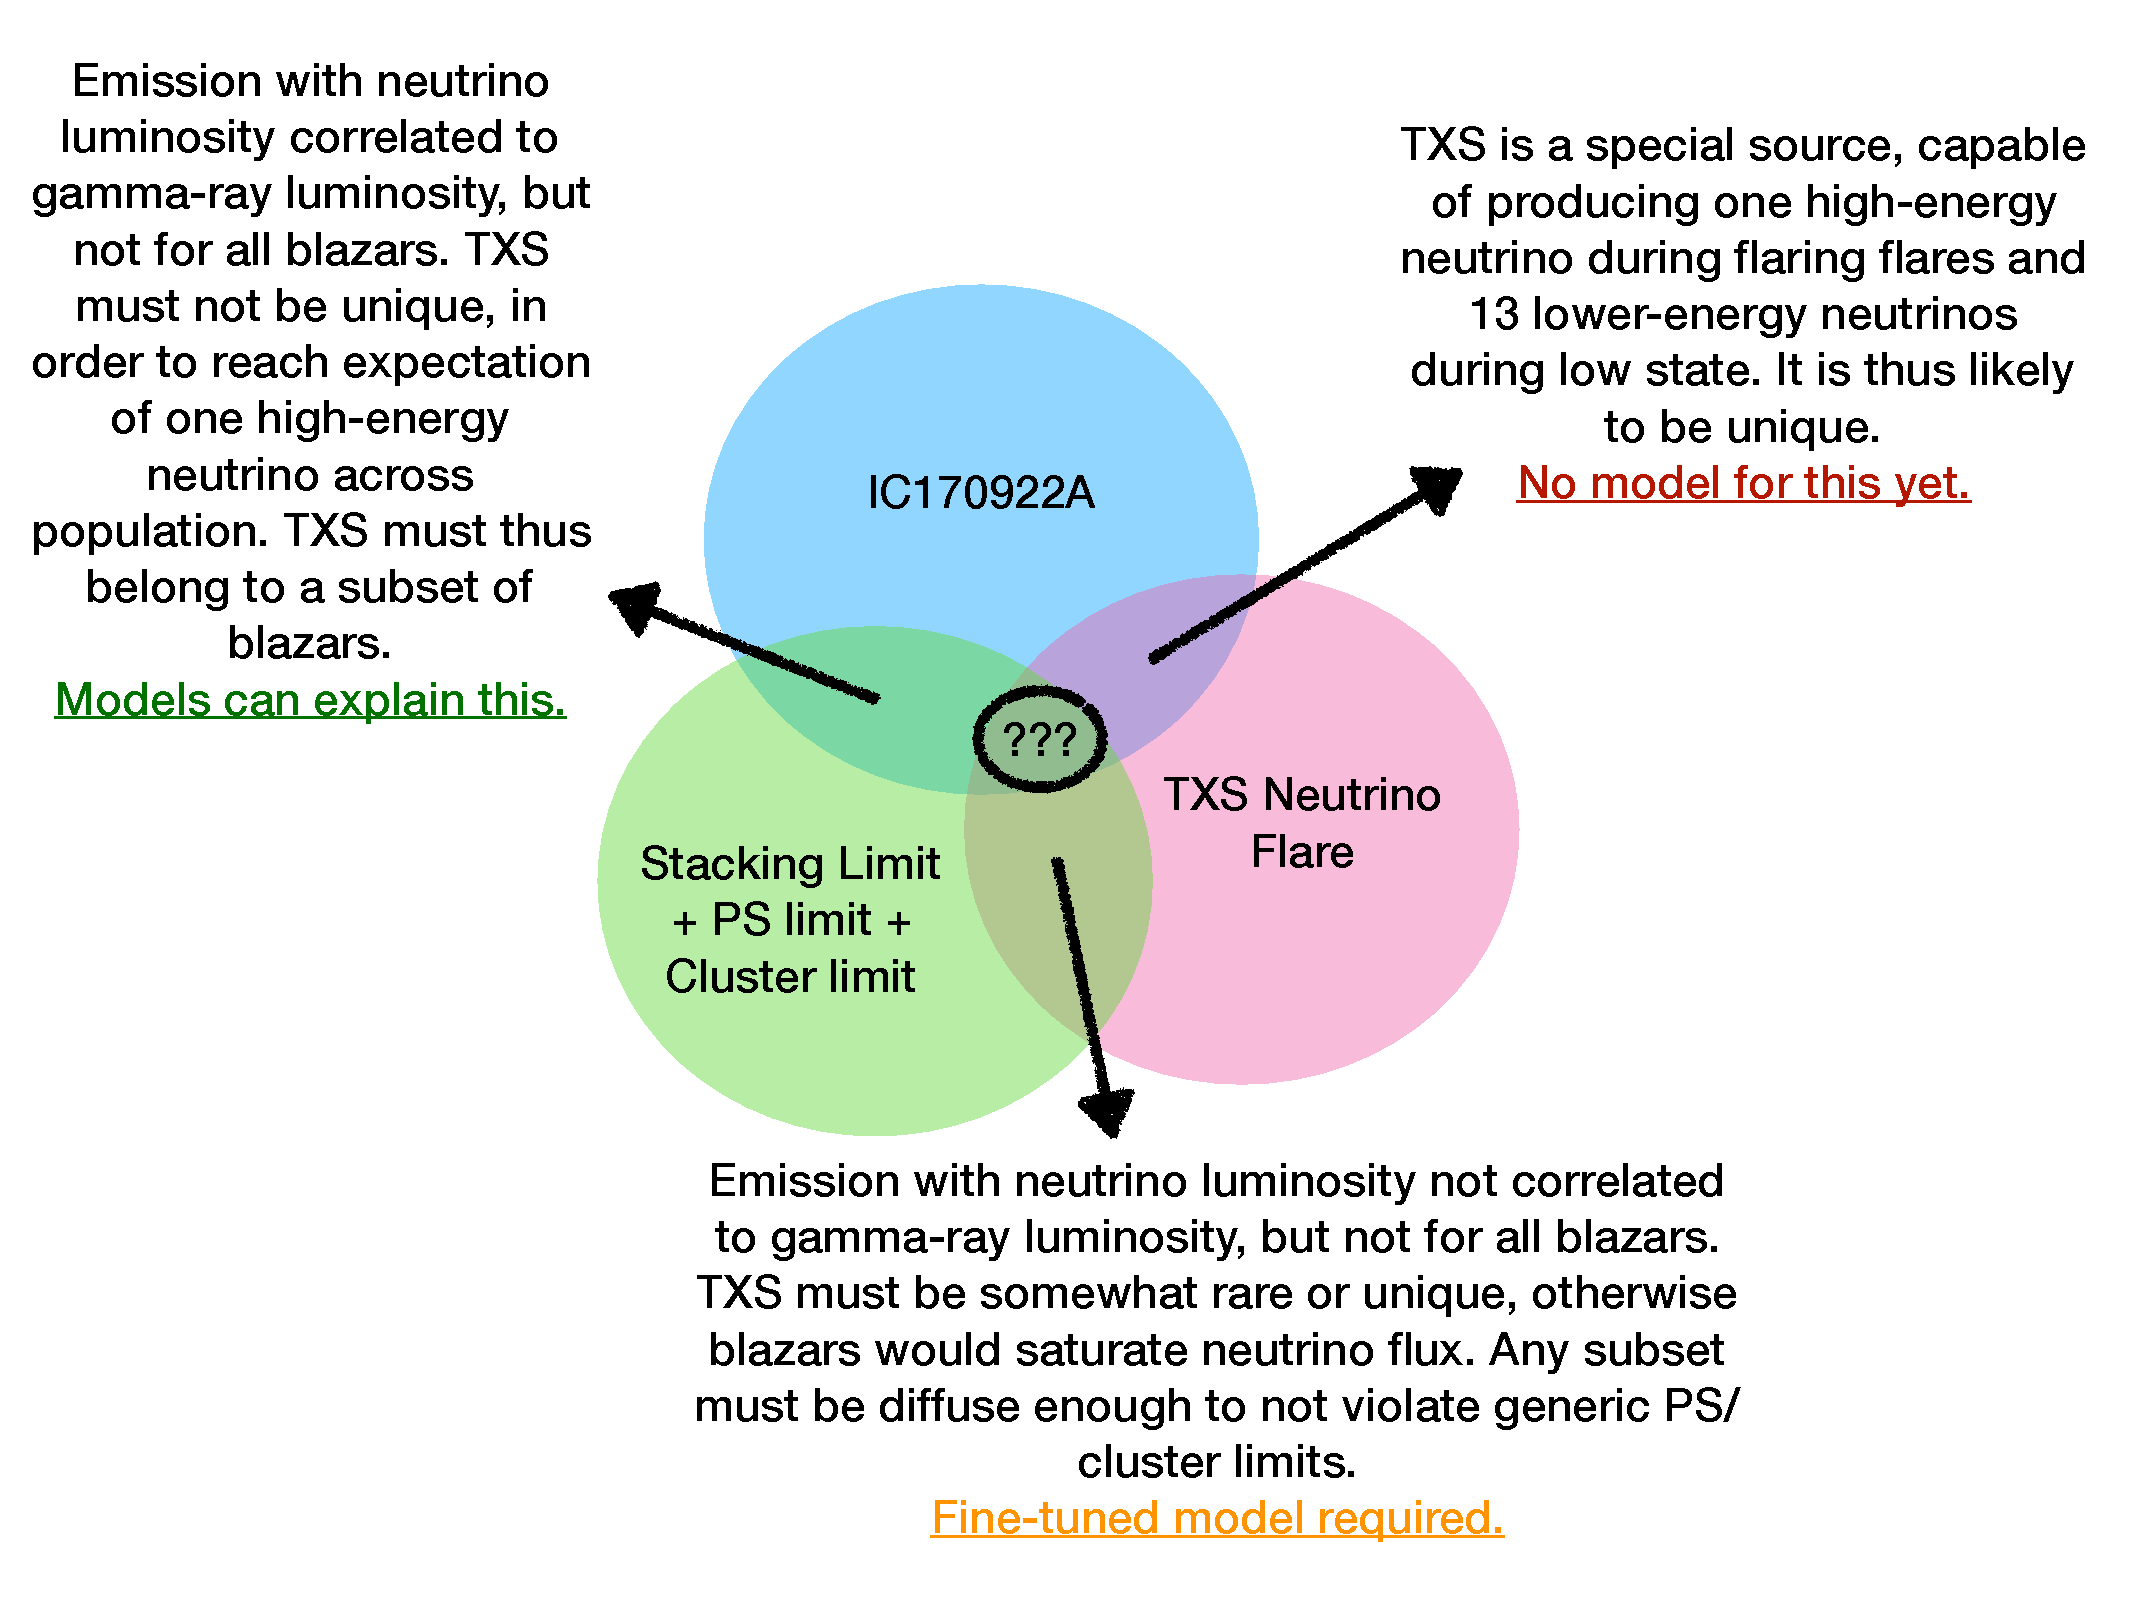
\includegraphics{txs_logic}
 	\caption{The challenge of coherently understanding the scenarios for neutrino emission from blazars, given the two pieces of evidence from TXS 0506+056, as well as the constraints from IceCube stacking analyses, general point-source searches and generic time-dependent cluster searches. To date, no model has resolved all three observations coherently.}
 	\label{fig:TXSLogic}
 \end{figure}
\section{Gamma-Ray Bursts}

Gamma-ray Bursts (GRBs) have long been proposed as a source of neutrinos. GRBs themselves fall into two broad categories, short and long, which are believed to arise from distinct physical populations. Long GRBs have been associated with the appearance of broad-lined type Ic supernova, and are thus believed to arise from a relativistic jet produced during supernova explosion. 

Short GRBs are now known to arise from relativistic jets launched during the merger of binary neutron stars. The first, and to date only, observed coincidence occurred for the gravitational wave event GW170817, which was associated with the short GRB 170817A and the kilonova AT2017gfo. Observations of GRB170817A revealed that it was particularly underluminous relative to most short GRBs, a fact later explained by comprehensive observations and modelling of AT2017gfo that confirmed an off-axis jet geometry. Given the relatively narrow jet opening angle, it is expected that the majority of future binary neutron star mergers detected by LIGO will not have detectable GRB counterparts.

Afterglow for both?

For both short and long GRBs, neutrino emission might be expected during the so-called "prompt phase" of gamma-ray emission. IceCube has undertaken numerous searches for neutrino emission, but has so far observed no correlation. Prompt emission from GRBs is particularly favourable for neutrino detection, because the brief and well-defined search period greatly reduces the expected background for such searches. This scenario is indeed one of the most-constrained by IceCube, which current limits restrict to less than 1\% of the astrophysical neutrino flux. 

Our understanding of GRBs has recently expanded further after the discovery of GRB VHE gamma-ray emission by MAGIC and HESS collaborations. The timescales for this emission, extending as much as 18 days after prompt phase indicates that high-energy processes extend throughout the so-called afterglow phase. consequently there is renewed focus on potential neutrino afterglow  emission, which is significantly less-constrained. One previous Icecube analysis limited the contribution to n\% (cite HESE).

An additional subclass are so-called low-luminosity GRBs (LLGRBs), believed to be... Given the poor efficiency with which source sources are detected, stacking searches of LLGRBs are significantly less powerful. However, for this case, generic searches for short-scale neutrino multiplets provide constraints on the contribution of such a population. In this case, they are known to contribute less than x\%.
\section{Core-Collapse Supernova}
 \begin{marginfigure}
	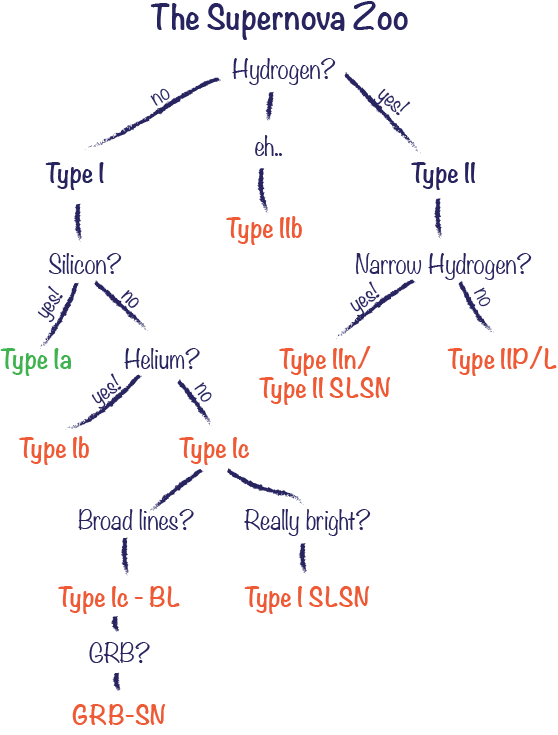
\includegraphics{sn_zoo-1}
	\caption{An overview of the current supernova classification scheme, which has been recently expanded to include superluminous supernova. Type 1a supernovae, marked in green, arise from thermonuclear explosions. All other classes, marked in origin, occur due to core collapse.}
	\labfig{fig:snzoo}
\end{marginfigure}
Supernovae, the explosive death of stars, are perhaps the best-studied phenomenon in astronomy. They are traditionally classified based on observed properties, rather than intrinsic physical attributes. An overview of a classification scheme is given in Figure \ref{fig:snzoo}. The most fundamental distinction is in explosion mechanism, with Type 1a SNe occuring due to thermonuclear explosions while all other classes are believed to arise from stellar core collapse. Further distinctions are made based on emission line, yielding the classes of Type Ib, Ic and Type II. Some SNe are observed to have narrow lines, which occur due to interaction with ejecta and circumstellar material (CSM). These supernova are denoted with 'n', the most common being Type IIn. This group in particular are candidate neutrino sources, in which neutrinos are produced via CSM interactions. An additional class of SNe is the IIP subclass, the subset of Type II SNe for which a characteristic lightcurve plateau is observed. Such plateaus are typically assumed to arise from....
Those Type II supernova not falling into IIp are instead classified as IIL, with characteristic Linear decay lighcurves.

Type Ic SNe can occasionally be observed with spectroscopic features known as Broad-Lines, which typically indicate the presence of fast-moving material. These form a distinct sublass, and it is this subclass which has been associated with long GRBs. Though radio observations have excluded the possibility that all Ic-BL SNe host relativistic jets? it is expected that even those without an observed GRB may instead host so-called 'choked jets' . These occur if a relativistic jet is lauched during core collapse, but because it lacks sufficient power to break through the outer layers of stellar material, it is stopped within the interior of the star. These choked jets, much like their standard counterparts, could produce neutrino emission. This scenario is however particularly difficult to test, because only those choked jets aligned towards Earth would produce a neutrino signal. As the alignment of a choked jet cannot be measured, it is impossible for us to say which supernova should or should not produce neutrinos. 

An additional category of supernovae has been recently observed, identifiable by their atypical brightness. So-called Superluminous supernovae (SLSNe) were initially classified as any SNe with an absolure magnitude brighter than -21 mag. However, in recent years, increased study has led to a spectroscopic classification being favoured, with some dimmer objects in the range $-20 < M < -21$ also being accepted. There are currently two favoured models to explain why SLSNe are so bright, namely the Magnetar model and the PISN model. .....

\section{Tidal Disruption Events (TDEs)}
== Roche Limit==
The tidal radius can best be understood by comparison to the more straightforward concept of the Roche Limit, otherwise known as the Roche Radius. The Roche Radius is defined as the distance at which the self-gravitiational force acting on the outer surface of a body are exactly equal to the gravitational pull of a second body on that same mass element. If a star moves closer than its Roche Radius for an SMBH, there will be a net force on mass elements on the star surface towards the SMBH, and the star will disintegrate.

The Tidal Force of one body acting on another is simply the difference in gravitational force strength between the closer surface of the sphere and its core. The Tidal Force of a black hole of mass M and distance d, acting on a mass element u lying on the closest point of the stellar surface, is thus given by:

$F_{tidal} = \frac{GMu}{(d-r)^{2}} - \frac{GMu}{(d)^{2}}$

$F_{tidal} = \frac{GMu}{d^{2}}((1-\frac{r}{d})^{-2} - 1 )$

Using Binomial Expansion with the reasonable assumption that r<<d, we reach an approximation:

$F_{tidal} \approx \frac{GMu}{d^{2}}\times \frac{2r}{d}$
The Roche Radius for a black hole of mass M for a star of mass m and radius r is thus found by equating this with the self-gravitational force acting on the same mass element. 

$F_{grav} = \frac{Gmu}{r^{2}} = \frac{2GMur}{d^{3}} \approx F_{tidal}$

$ d = r \times (\frac{2M}{m})^{\frac{1}{3}} \approx r_{roche}$

== Tidal Radius ==

This simplistic model does not hold for Tidal Disruption Events. The tidally-disrupted body would need to be in a circular orbit with synchronised spin, but stars tend to have approach Black Holes parabolically. In addition to Angular Momentum, General Relativity should be accounted for. This is particularly relevant for large black holes. A rigorous definition of Tidal radius should account for these things, but in any case, the point at which a star becomes 'tidally disrupted' is difficult to define. An event which only strips a fraction of the outer shell of the star would be ambiguous. Fortunately these definitions differ only by the order of unity from the Roche Radius. In the original paper introducing these calculations by [https://www.nature.com/nature/journal/v333/n6173/abs/333523a0.html Rees (1988)], the tidal radius was defined as the radius at which the mean internal density of the star is exceed by the mean internal density of the orbital volume. In this definition:

$\rho_{star} = \frac{m}{\frac{4}{3} \pi r ^{3}}  = \frac{M}{\frac{4}{3} \pi d ^{3}}= \rho_{volume}$

$ d = r \times (\frac{M}{m})^{\frac{1}{3}} = r_{tidal} $

Thus we see that:

$ r_{tidal} = \frac{r_{roche}}{\sqrt[3]{2}} $

In any definition of a characteristic tidal radius, we nonetheless always find that the radius scales with the cubic root of mass. It is interesting to recall that, in contrast, the Schwarzschild Radius of a black hole scales linearly with its mass. 

$R_{S} = \frac{2GM}{c^{2}}$

Consequently, the Schwarzschild Radius of the Black Hole grows faster as a function of Mass than the tidal radius. There is thus a critical black hole mass, for which the Schwarzschild Radius equals the star's Tidal Radius. Above this, a TDE cannot occur, because the star would have to be wholly swallowed by the black hole in order to be tidally disrupted. Though the exact limit will vary somewhat depending on the mass of the star, using typical values gives us an order-of-magnitude upper limit on TDE-generating black holes of $M < 10^{8} M_{\odot}$.

== Post-Disruption Evolution ==

For TDEs, the accretion of stellar material produces a highly-luminous flare, which is often the cause of discovery. This can be visible in Optical, UV or XRays. The bound mass spirals into the Black hole, but the fall-in time of each mass element in the bound material depends on the Gravitational Potential Energy of the element, leading to a characteristic fall-in rate $ \frac{dM}{dt} \propto t^{\frac{5}{3}}$ relation. This, in turn, can be seen in the light curves of TDEs.

There is evidence to support the existence of jetted TDEs, and these are usually highly-luminous in X rays. However, the classification of candidates into jetted or non-jetted can be unclear.

There is a further proposed model in which an envelope forms around the Black Hole, which could lead to choked jets.

== Neutrino Emission ==

The process for neutrino emission in TDEs, as well as the expected rates and neutrino light curves, are all highly uncertain. A key component of this analysis will be to probe the importance of an accurate time PDF, and the degree to which a minimal-assumption wide box model is the optimal time PDF to use. Even assuming the shape of the expected light curve was well known for each TDE (either the same neutrino light curve for every TDE,  or one closely correlated to the TDE optical or X Ray light curve), there remains a sigificant degree of uncertainty regarding the delay between neutrino emmision and optical emmission. It is possible that the peak neutrino emission is achieved more than 100 days before optical peak, but the expected gap is entirely model-dependent. The following potential models have been proposed for Neutrino Acceleration:

* Jetted TDEs, such as Swift J1644-57
* Choked Jet Scenario

Tidal Disruption Events (TDEs) are rare transients that occur when stars pass close to supermassive black holes (SMBHs). Studies have suggested that TDEs are sources of high-energy neutrinos and ultra-high energy cosmic rays\cite{2009ApJ...693..329F,2017MNRAS.469.1354D}, in particular those TDEs with relativistic particle jets\cite{2014arXiv1411.0704F,2017ApJ...838....3S,2016PhRvD..93h3005W,2017PhRvD..95l3001L}. TDEs with non-thermal radio emission are considered the most likely candidates for sources of high-energy neutrinos.

\section{Fast Radio Bursts}

A relatively recent astro

\section{Active Galactic Nuclei and Starburst Galaxies}
One additional possibility is that the astrophysical neutrino flux is produced by a large population of steady sources, and is thus truly a \textbf{diffuse} astrophysical neutrino flux. One case would be for neutrino production in Starburst Galaxies, which has been suggested in various models x.

Starburst galaxies are those galaxies for which there is a high level of star formation. Such galaxies have elevated supernovae rates, and are typically bright in UV and such. Starburst galaxies have been detected in gamma rays, including at very high energies, confirming the existence of acceleration processes. A search for neutrino emission from Starburst Galaxies was performed in x, and no significant correlation was identified. Given the expected dominant contribution from unresolved Starburst galaxies to any population neutrino flux, and accounting for the fact that this aggregate flux must not exceed the measured astrophysical neutrino flux, it is clear that the nearby starburst galaxies must therefore be very weak neutrino emitters. Such a scenario is unfavourable for identification against an isotropic neutrino background, and in this case it is unlikely that IceCube would have sufficient sensitivity to identify the neutrino flux origin.

A similar case would occur in that case of neutrino production from the cores of Active Galactic Nuclei (AGN), as suggested by XYZ. Here neutrinos would arise from pn interaction occurring in the inner accretion disk of AGN, with the corresponding gamma-ray emission being absorbed. Such a scenario is appealing theoretically, as it would neatly evade the existing constraints on diffuse gamma-ray emission, which we know to arise predominantly from blazars. This hypothesis was tested by IceCube (I hope...)

SUMMARY TABLE with source class, limit, and spectral index